%% Identified supplementary material for WSDM 2027 paper 2126
%% Build with latexmk -pdf supplement.tex
\documentclass[manuscript,nonacm]{acmart}
\usepackage{booktabs}
\usepackage{graphicx}
\usepackage{enumitem}
\usepackage{placeins}
%% amssymb is already loaded by acmart
\settopmatter{printacmref=false}
\setcopyright{none}
\acmConference[WSDM '27]{Supplementary material}{February 15 to 19, 2027}{Hong Kong SAR, China}
\newcommand{\system}{VoI-Search}
\newcommand{\fbgpred}{\widehat{\mathrm{FBG}}}
\hypersetup{pdftitle={Supplement: A Selection-Aware Audit of Learned Stopping in Short-Horizon Iterative Retrieval}}


\begin{document}
\title[Supplement: Selection-Aware Stopping Audit]{Supplementary Material: A Selection-Aware Audit of Learned Stopping in Short-Horizon Iterative Retrieval}
\author{Xuan-Bach Le}
\orcid{0009-0003-6848-5403}
\affiliation{\institution{Ho Chi Minh City University of Technology (HCMUT), VNU-HCM}\city{Ho Chi Minh City}\country{Vietnam}}
\email{lexuanbach@hcmut.edu.vn}
\author{Phat T. Tran-Truong}
\orcid{0000-0003-3199-6333}
\affiliation{\institution{Ho Chi Minh City University of Technology (HCMUT), VNU-HCM}\city{Ho Chi Minh City}\country{Vietnam}}
\email{phatttt@hcmut.edu.vn}
\author{Son Ha Xuan}
\orcid{0000-0002-5336-0566}
\affiliation{\department{The Business School}\institution{RMIT University}\city{Ho Chi Minh City}\country{Vietnam}}
\email{ha.son@rmit.edu.vn}

\author{Duy Nguyen}
\orcid{0009-0000-6348-8830}
\affiliation{\institution{University of Economics Ho Chi Minh City}\city{Ho Chi Minh City}\country{Vietnam}}
\email{duynguyen.726202321440@st.ueh.edu.vn}
% Duy Nguyen ORCID supplied directly by the corresponding author.
% Names follow the author's WSDM listings. Synchronize CMT/ACM before submission.

\maketitle

This supplement preserves the complete per-cell displays and diagnostics
behind the main paper. Every generated value comes from the identified
artifact's retained trajectories. Section references point to the main paper.
Policy codes are F$k$ for fixed budget $k$, Rep for answer repetition, TASR for
full TASR with native log probabilities, NLI for FBG with an NLI feature and
repeat guard, Clf for the binary future-improvement classifier, Err for the error-head
gate, StopRAG for a cell-trained Stop-RAG model, V for FBG-only, and G for
guarded FBG. Unless a caption states otherwise, entries report exact-match
percentage and exact LLM calls. D denotes domination by a simple policy. F
denotes a frontier point that does not strictly improve the selected
$B^\star$. I denotes an undominated point that strictly improves $B^\star$.
Dom(G) lists policies dominating G, lb is a one-sided lower bound, CI is a
95\% confidence interval, and NA means that an analysis is unavailable.
In the archived call-only panels, \system{} denotes the deployed guarded FBG
controller.

\section{Proof sketch for the certificate risk bound}

Fix one target risk $\alpha$ and let
$L=\lceil\log_2 m\rceil$. Because the stopping rule and error score are fixed
before calibration, each episode contributes one independent stopped-state
score and error pair. We group equal scores, which gives a nested family of
candidate sets in $q$ and prevents a threshold from splitting a tie group.
Binary search queries at most $L$ candidates. For a queried candidate with
$n_q$ examples and $k_q$ errors, we use the one-sided Clopper and Pearson upper
bound
\[
U_q=\operatorname{Beta}^{-1}_{k_q+1,n_q-k_q}\!\left(1-\frac{\delta}{L}\right),
\]
with $U_q=1$ when $k_q=n_q$. The exact binomial coverage and a union bound over
the queried candidates imply that every queried bound is valid jointly with
probability at least $1-\delta$. The nonempty subset returned by SGR therefore
has risk at most $\alpha$ whenever $U_q\le\alpha$. If no candidate passes, our
procedure returns no certificate. We run this construction separately for the
six reported $\alpha$ values and make no joint $1-\delta$ claim across them.

\paragraph{Excluded score-mismatch diagnostic.}
Nine call-only cells predate retention of deployment-matched stopped-prefix
features. Their archived diagnostic calibrates on cross-fitted scores but
evaluates full-fit scores, so calibration and test scores do not share the
same construction. Thirteen of 54 cell and target-risk pairs appear to fire
under this mismatched procedure. We quarantine all 54 values and exclude them
from certificate evidence. This is why the main decision matrix marks these
cells NA and the formal result uses only the 14 cells with a dedicated split
and deployment-matched scores.

\section{Evidence hierarchy}
\label{supp:hierarchy}

\begin{table}[H]
\caption{Claim-to-evidence hierarchy and the inference licensed by each row.}
\label{tab:hierarchy}
\footnotesize
\setlength{\tabcolsep}{3pt}
\begin{tabular}{p{0.28\columnwidth}p{0.44\columnwidth}p{0.20\columnwidth}}
\toprule
Claim & Evidence population & Status \\
\midrule
Guarded FBG passes the declared full-search comparison & One 400-question
HotpotQA corpus cell with EM and exact calls & Primary endpoint \\
FBG has no resolved matched-cost gain & 18-cell calls family, 14-cell token
and wall-time family, and answer-once ledger & Robustness \\
Question sampling can change the endpoint decision & Same-question reruns and
four independent question draws & Prospectively frozen \\
Signal role and selection explain the frontier gap & Alternative heads,
calibration, rerolled futures, nested reselection, and oracle & Exploratory
diagnosis \\
The certificate refuses unsupported subsets & 84 cell and target-risk pairs
over 14 fully instrumented core cells & Robustness \\
\end{tabular}
\end{table}

\section{Regime-specific policy guidance}
\label{supp:headline-displays}

\begin{table}[H]
\caption{Regime-specific policy guidance supported by the evaluated cells.}
\label{tab:supp-decision}
\footnotesize
\setlength{\tabcolsep}{4pt}
\begin{tabular}{p{0.29\columnwidth}p{0.31\columnwidth}p{0.31\columnwidth}}
\toprule
Observed regime & Evidence in this study & Practical decision \\
\midrule
Accuracy saturates by the second search & An FBG-family rule is the cheapest
policy within 1 EM of full search in 1 of 14 fully instrumented core cells &
Select fixed-2 or repetition on development data \\
Large shared index with cross-document negatives & Fixed-2 reaches 23.0 EM at
5.00 calls and dominates guarded FBG at 21.25 EM and 5.90 calls & Prefer the
selected fixed budget \\
Question populations have heterogeneous saturation & Guarded FBG passes on
some independent draws and fails on others & Validate on a new question draw
before deployment \\
The selected threshold lies at the grid boundary & FBG-only can collapse while
the latched guard reduces to answer repetition & Treat the score as unstable
and require a new equal-cost test \\
Calibration has only 30 episodes & Corrected SGR returns no certified subset
for targets through 0.6 & Report zero coverage rather than a weak certificate \\
Evidence sufficiency is predictable & Gold-support AUROC reaches 0.65 to 0.95,
yet no cell has a positive cellwise equal-call interval & Do not infer policy
utility from target discrimination alone \\
\bottomrule
\end{tabular}
\end{table}

\section{External news-corpus extension}
\label{supp:external}

We wrote the MultiHopRAG endpoint protocol before fitting the external cell or
evaluating its 400 test questions. The adapter retains inference queries and
indexes 53{,}943 sentence units from all 609 English news articles. It excludes
comparison, temporal, and null queries under the declared answer-format rules.
The cell uses Qwen2.5-3B, 96 policy-training episodes, 24 certificate episodes,
and the same four-search cap as the primary HotpotQA corpus cell.

\begin{table}[htbp]
\caption{External-cell policies and equal-call differences from the randomized
simple-policy hull.}
\label{tab:supp-external}
\small
\begin{tabular}{lrrrl}
\toprule
Policy & EM & Calls & $\Delta$EM & 95\% CI \\
\midrule
FBG-only & 73.00 & 7.27 & $+0.48$ & $[-0.50,1.46]$ \\
Guarded FBG & 73.25 & 7.40 & $+0.71$ & $[-0.07,1.57]$ \\
Stop classifier & 70.50 & 4.35 & $+2.10$ & $[0.12,4.10]$ \\
Error-head gate & 73.75 & 7.65 & $+1.18$ & $[0.41,2.06]$ \\

\bottomrule
\end{tabular}
\end{table}

Guarded FBG meets its prospectively frozen comparison with full search because
its paired difference is $+0.50$ EM $[0.00,1.25]$ and calls fall from 9.00 to
7.40. Its equal-call interval remains unresolved. The two positive intervals
for the exploratory signal policies are separate from the frozen endpoint
because neither policy was the frozen
external endpoint. We also lack gold support aligned to this adapter, so the
gold-support sufficiency classifier is not eligible in this cell.


\section{Signal calibration and evidence sufficiency}
\label{supp:signal-audit}

We evaluate target quality separately from policy quality on the 18-cell common
family. At each test prefix, the error head has expected calibration error from
0.019 to 0.087 with median 0.043. Its selective-risk ordering improves over a
random ordering in all 18 cells. The FBG value head improves over random in 7
of 18. These diagnostics use test labels only for evaluation and do not change
any threshold or stopping time.

The gold-support classifier marks a prefix sufficient when the retained
evidence covers at least 0.8 of annotated support tokens. Gold support is read
during training only. With the nine controller features, cross-fitted AUROC
ranges from 0.652 to 0.946. This policy is in category D in 8 cells, F in 8,
and I in 2. A twelve-feature lexical variant has AUROC from 0.629 to 0.945 and
categories 9/7/2 in D/F/I order. Neither variant has a cellwise positive
equal-call interval. We therefore interpret target discrimination as evidence
about the signal, not as evidence that the selected policy improves the
simple-policy frontier.

\section{Positioning against the closest stopping methods}
\label{supp:related}

We use “matched” when a policy replays identical trajectories and shares our
call accounting. We use “transplanted” when a released system retains its own
retriever or generation schedule on the baseline-implementation cell. “Not
run” identifies a declared missing condition. Our matched rows use a sparse
first-stage retriever, so they do not support claims about dense retrieval.
We price transplanted methods in \emph{searches} because their per-question
LLM-call counts are not comparable with our exact-call ledger.

The controlled deterministic family contains fixed budgets and answer
repetition. Retrieval-score saturation, semantic novelty, query repetition,
context growth, grounding thresholds, and cheap-controller cascades remain
separate comparator families. Several enter our learned feature set, but we do
not treat that use as a standalone tuned heuristic. The main-paper frontier
claim is therefore relative to the declared family in the final row below.

\begin{table}[htbp]
\caption{Signals, requirements, matched conditions, and measured outcomes for
the closest stopping and adaptive-retrieval methods.}
\label{tab:supp-related}
\small
\setlength{\tabcolsep}{4pt}
\begin{tabular}{p{1.9cm}p{2.1cm}p{2.6cm}p{2.9cm}p{3.9cm}}
\toprule
Method & Stop signal & Needs, action space, backend & Comparison here & Outcome in this audit \\
\midrule
Stop-RAG~\cite{park2025stoprag} & Q($\lambda$) stop and continue values & logged trajectories and encoder training & matched on 14 common-family cells with cell-specific retraining & dominated in 9 cells, frontier-only in 4, and improves the selected fixed budget in 1 \\
TASR~\cite{kieback2026tasr} & answer stability and calibrated logits & native answer-token log probabilities & matched on 11 of 14 fully instrumented core cells & nondominated in 2 of 11 and point-dominated by FBG-only in the primary cell \\
HALT~\cite{roh2026halt} & generated-claim coverage & claim generator and trained verifier & verifier-inspired substitute on six cells & dominated in all six cells under both public substitute verifiers, by fixed-2 in five \\
SIM-RAG~\cite{yang2025simrag}, S2G-RAG~\cite{li2026s2grag} & evidence sufficiency & learned sufficiency supervision & related signal only & motivates our separate gold-support classifier \\
Gold-support classifier & support-token coverage & gold support during training only & matched on 18 cells & cross-fit AUROC 0.65 to 0.95 with no cellwise equal-call win \\
Error-head gate & current answer error & correctness labels & matched on 18 cells & one cellwise equal-call win and no max-t-resolved win \\
LearnStop~\cite{dong2026learnstop} & learned exit versus scalar rules & analysis conditions & organizing hypothesis & early saturation and scalar reliability motivate our diagnostics \\
Self-RAG~\cite{asai2024selfrag} & reflection tokens & fine-tuned model with its own dense retriever & transplanted released 7B system & 7.9~EM at 0.56 searches on the baseline-implementation cell \\
FLARE~\cite{jiang2023flare} & token-probability uncertainty & mid-generation retrieval and native logits & transplanted direct system & 34.3~EM at 1.66 searches on the baseline-implementation cell \\
Fixed budgets and repetition & deterministic budget or answer stability & no learned predictor & primary matched comparator in every cell & guarded FBG is dominated in 15 of the 26 core cells \\
\bottomrule
\end{tabular}
\end{table}

\FloatBarrier
\section{Pooled frontier, Stop-RAG, and margin sensitivity on fully instrumented cells (RQ1)}

\begin{table}[!htbp]
\caption{Fourteen-cell frontier summary with nondominated counts, cheapest
policies within 1/2/3 EM, and mean matched-cost differences.}
\label{tab:supp-whowins-instrumented}
\footnotesize
\setlength{\tabcolsep}{2.5pt}
\begin{tabular}{@{}lccrrr@{}}
\toprule
& & Band & \multicolumn{3}{c}{$\Delta$EM at equal cost} \\
\cmidrule(lr){4-6}
Policy family & Nondom. & 1/2/3 & calls & tokens & wall \\
\midrule
Fixed budgets & 12 of 14 & 4/7/9 & NA & NA & NA \\
Answer repetition & 5 of 14 & 1/0/0 & NA & NA & NA \\
\midrule
FBG-only & 11 of 14 & 0/2/1 & $+0.01$ & $-0.02$ & $+0.02$ \\
FBG + repeat guard & 3 of 14 & 0/0/0 & $-0.59$ & $-0.64$ & $-0.60$ \\
FBG + NLI guard & NA & 1/0/0 & NA & NA & NA \\
\midrule
Stop classifier & 13 of 14 & 5/5/4 & $-0.06$ & $-0.07$ & $-0.06$ \\
Full TASR & 2 of 11 & 2/0/0 & $-0.32$ & $-0.34$ & $-0.33$ \\
Stop-RAG & 5 of 14 & NA/NA/NA & $-1.20$ & NA & NA \\
Error-head gate & 3 of 14 & 0/0/0 & $-0.47$ & $-0.47$ & $-0.48$ \\
Verifier-inspired coverage & 0 of 6 & 0/0/0 & NA & NA & NA \\

\bottomrule
\end{tabular}
\end{table}

Denominators follow signal eligibility. Stop-RAG has equal-call vectors for
fourteen cells, but its complete token, wall-time, and all-policy band ledgers
are unavailable. We report those entries as NA.

\begin{table}[htbp]
\caption{I/F/D counts across the 26 core cells under
$\epsilon$-dominance. The zero tolerance matches the point matrix.}
\label{tab:supp-epsilon}
\small
\begin{tabular}{lcc}
\toprule
$\epsilon$ (EM) & FBG-only I/F/D & Guarded FBG I/F/D \\
\midrule
0 & 3/13/10 & 5/6/15 \\
0.5 & 2/9/15 & 4/4/18 \\
1 & 0/8/18 & 1/2/23 \\
2 & 1/5/20 & 0/1/25 \\

\bottomrule
\end{tabular}
\end{table}


\label{supp:pooled}

The core matrix assigns guarded FBG to category I in five cells. These are
Sonnet 4.5, the call-only Qwen and MuSiQue with Llama cells, and independent
corpus draws D and E. Category D includes GPT-oss-120B, Command-R, two of the
three same-question runs, the Wikipedia boundary cell, and all three 2Wiki
draws. The remaining six cells are frontier-only and need not be accuracy
ties.

For the target comparison below, ``logged'' is the deployed run and ``refit''
reruns the same pipeline with seeded tie-breaking. The net and discounted
targets use $\max_{t'>t}[u_{t'}-u_t-c(t'-t)]_+$ and
$\max_{t'>t}\gamma^{t'-t}[u_{t'}-u_t]_+$, respectively. Clf is a
binary future-improvement classifier. Err thresholds the error head. All thresholds
use the frozen band rule on cross-fitted training chains.

\begin{table}[htbp]
\caption{Guarded-policy EM/calls and verdicts under alternative targets and
learners.}
\label{tab:supp-targets}
\footnotesize
\setlength{\tabcolsep}{2.5pt}
\begin{tabular}{lrrrrrrrrrr}
\toprule
Run & FBG (logged) & FBG (refit) & net $c{=}.02$ & net $c{=}.04$ & net $c{=}.08$ & disc.\ $\gamma{=}.5$ & disc.\ $\gamma{=}.8$ & one-step & Clf & Err \\
\midrule
A s7 & 24.8/6.75\,F & 24.8/6.75\,F & 24.8/6.77\,F & 24.5/6.67\,D & 24.5/6.65\,D & 25.0/6.64\,I & 24.5/6.56\,D & 25.0/6.70\,I & 24.5/5.11\,D & 24.5/8.79\,D \\
A s11 & 25.2/6.50\,D & 25.0/6.90\,D & 24.8/6.90\,D & 25.2/6.88\,D & 25.5/6.84\,D & 25.0/6.36\,D & 25.5/6.75\,D & 24.5/6.40\,D & 25.8/4.96\,I & 25.0/8.89\,D \\
A s19 & 25.5/6.67\,D & 25.5/6.67\,D & 25.8/6.63\,F & 25.8/6.66\,F & 26.0/7.07\,D & 25.8/7.04\,D & 26.0/7.05\,D & 26.2/6.95\,I & 24.0/4.94\,F & 26.0/8.88\,D \\
B & 29.2/6.71\,F & 28.0/5.96\,D & 28.2/5.83\,D & 28.2/5.82\,D & 27.8/5.83\,D & 27.8/5.75\,D & 28.0/5.80\,D & 28.2/5.89\,D & 27.8/4.96\,F & 30.2/7.70\,D \\
C & 23.2/5.90\,F & 23.2/5.90\,F & 23.2/5.90\,F & 23.2/5.90\,F & 23.2/5.90\,F & 23.2/5.90\,F & 23.2/5.90\,F & 23.2/5.90\,F & 18.5/3.91\,F & 26.5/8.84\,F \\
D & 27.0/6.36\,I & 26.5/5.89\,D & 26.5/5.89\,D & 26.5/5.89\,D & 26.5/5.89\,D & 26.5/5.89\,D & 26.5/5.89\,D & 26.5/5.89\,D & 25.5/4.96\,I & 26.0/8.63\,D \\
E & 34.2/7.75\,I & 34.2/7.75\,I & 34.0/8.21\,F & 34.0/8.20\,F & 34.0/8.15\,F & 34.2/7.62\,I & 32.5/5.86\,F & 34.2/6.86\,I & 27.2/4.00\,F & 34.0/8.67\,F \\
2Wiki d1 & 23.5/5.50\,D & 23.5/5.50\,D & 23.5/5.50\,D & 23.5/5.50\,D & 23.5/5.50\,D & 23.5/5.50\,D & 23.5/5.50\,D & 23.5/5.50\,D & 23.5/4.11\,F & 23.5/6.79\,D \\
2Wiki d2 & 23.5/5.59\,D & 24.0/7.32\,D & 23.8/7.33\,D & 23.8/7.26\,D & 23.2/6.66\,D & 23.2/5.51\,D & 23.8/7.05\,D & 23.2/5.51\,D & 19.2/4.14\,F & 25.2/9.00\,D \\
2Wiki d3 & 25.8/5.66\,D & 25.8/5.82\,D & 25.8/5.81\,D & 25.8/5.66\,D & 25.8/5.66\,D & 25.2/5.61\,D & 25.5/5.64\,D & 25.5/5.66\,D & 25.2/3.79\,F & 25.8/8.74\,D \\
MuSiQue d1 & 7.5/6.54\,D & 7.5/6.54\,D & 7.5/6.53\,I & 7.5/6.53\,I & 7.5/6.53\,I & 7.5/6.53\,I & 7.5/6.53\,I & 7.5/6.53\,I & 5.2/3.41\,F & 9.2/9.00\,F \\
MuSiQue d2 & 9.2/6.50\,D & 9.8/6.89\,D & 9.8/6.99\,D & 9.8/7.00\,D & 9.8/6.98\,D & 9.5/6.88\,D & 9.8/6.97\,D & 9.5/6.99\,D & 9.8/4.95\,F & 10.2/9.00\,F \\
MuSiQue d3 & 10.8/6.42\,D & 10.8/6.42\,D & 10.8/6.42\,D & 10.8/6.42\,D & 10.8/6.42\,D & 10.8/6.42\,D & 10.8/6.42\,D & 10.8/6.42\,D & 6.5/3.08\,F & 12.0/9.00\,F \\
Wiki 25M & 21.2/5.89\,D & 21.2/5.89\,D & 21.2/5.95\,D & 21.2/5.89\,D & 21.2/5.89\,D & 21.2/5.88\,D & 21.2/5.88\,D & 21.2/5.90\,D & 17.8/3.00\,F & 21.5/8.97\,D \\

\bottomrule
\end{tabular}
\end{table}

\begin{table}[htbp]
\caption{Same targets under the FBG-only rule (EM/calls and verdict).}
\label{tab:supp-targets-value}
\footnotesize
\setlength{\tabcolsep}{3pt}
\begin{tabular}{lrrrrrrrr}
\toprule
Run & FBG (logged) & FBG (refit) & net $c{=}.02$ & net $c{=}.04$ & net $c{=}.08$ & disc.\ $\gamma{=}.5$ & disc.\ $\gamma{=}.8$ & one-step \\
\midrule
A s7 & 25.0/6.35\,I & 25.0/6.35\,I & 25.0/6.37\,I & 24.8/6.26\,F & 24.8/6.24\,F & 25.5/6.20\,I & 25.0/6.12\,I & 25.2/6.27\,I \\
A s11 & 25.2/5.74\,D & 25.8/6.38\,D & 25.5/6.37\,D & 25.5/6.27\,D & 25.8/6.20\,D & 25.0/5.48\,D & 25.8/6.10\,D & 24.5/5.54\,D \\
A s19 & 25.2/6.38\,D & 25.2/6.38\,D & 25.5/6.32\,D & 25.5/6.34\,D & 25.8/6.87\,F & 25.2/6.88\,D & 25.8/6.86\,F & 26.0/6.83\,I \\
B & 29.5/6.62\,F & 27.8/4.23\,F & 28.0/4.04\,F & 27.8/4.03\,F & 27.2/3.96\,F & 7.0/1.00\,D & 26.8/3.87\,F & 27.8/3.96\,F \\
C & 13.5/2.67\,F & 13.5/2.67\,F & 13.5/2.67\,F & 13.0/2.65\,F & 11.0/2.16\,F & 6.5/1.00\,F & 11.0/2.16\,F & 6.5/1.00\,F \\
D & 26.2/5.42\,I & 19.5/3.07\,D & 19.5/3.06\,D & 19.8/3.08\,F & 19.5/3.06\,D & 19.5/3.04\,D & 19.5/3.03\,D & 16.8/2.68\,F \\
E & 33.2/7.51\,F & 33.2/7.51\,F & 33.0/8.03\,F & 33.0/8.01\,F & 33.2/7.96\,F & 33.8/7.25\,F & 26.5/3.42\,F & 33.8/6.46\,F \\
2Wiki d1 & 20.2/3.11\,F & 20.2/3.11\,F & 20.5/2.98\,F & 20.5/2.97\,F & 20.5/2.96\,F & 8.8/1.00\,F & 19.8/2.87\,F & 10.5/1.40\,F \\
2Wiki d2 & 19.0/3.83\,F & 23.2/7.05\,D & 22.5/7.01\,D & 23.0/6.97\,D & 21.8/6.20\,D & 6.0/1.01\,D & 22.5/6.70\,D & 6.0/1.02\,D \\
2Wiki d3 & 24.2/3.12\,F & 25.5/4.07\,F & 25.5/4.03\,F & 24.0/3.10\,F & 11.0/1.57\,F & 6.0/1.00\,F & 10.0/1.39\,F & 9.8/1.41\,F \\
MuSiQue d1 & 3.8/3.02\,F & 3.8/3.02\,F & 3.2/2.69\,F & 0.5/1.00\,F & 0.5/1.00\,F & 0.5/1.00\,F & 0.5/1.00\,F & 0.5/1.00\,F \\
MuSiQue d2 & 2.5/1.44\,F & 9.8/6.21\,D & 9.8/6.79\,D & 9.8/6.81\,D & 9.8/6.79\,D & 9.2/6.71\,D & 9.8/6.78\,D & 10.2/6.59\,I \\
MuSiQue d3 & 0.2/1.00\,F & 0.2/1.00\,F & 0.2/1.00\,F & 0.2/1.00\,F & 0.2/1.00\,F & 0.2/1.00\,F & 0.2/1.00\,F & 0.2/1.00\,F \\
Wiki 25M & 18.0/3.13\,F & 18.0/3.13\,F & 18.0/3.19\,F & 18.0/3.11\,F & 17.8/3.09\,D & 10.0/1.50\,F & 10.0/1.50\,F & 10.0/1.55\,F \\

\bottomrule
\end{tabular}
\end{table}

\begin{table}[htbp]
\caption{Paired EM difference from the randomized simple-policy frontier at
equal mean calls, input tokens, or wall time (95\% bootstrap CI).}
\label{tab:supp-equalcost}
\footnotesize
\setlength{\tabcolsep}{3pt}
\begin{tabular}{lrrrrrr}
\toprule
& \multicolumn{3}{c}{FBG + guard} & \multicolumn{3}{c}{FBG-only} \\
\cmidrule(lr){2-4}\cmidrule(lr){5-7}
Run & equal calls & equal tokens & equal wall & equal calls & equal tokens & equal wall \\
\midrule
A s7 & -0.19\,[-1.22,0.84] & -0.23\,[-1.35,0.79] & -0.20\,[-1.25,0.83] & +0.16\,[-0.85,1.17] & +0.14\,[-0.91,1.16] & +0.17\,[-0.84,1.17] \\
A s11 & -0.50\,[-2.50,1.25] & -0.50\,[-2.50,1.25] & -0.50\,[-2.50,1.25] & -0.50\,[-2.00,1.00] & -0.50\,[-2.00,1.00] & -0.50\,[-2.00,1.00] \\
A s19 & -0.37\,[-1.44,0.69] & -0.42\,[-1.55,0.66] & -0.37\,[-1.44,0.69] & -0.51\,[-1.88,0.84] & -0.52\,[-1.89,0.79] & -0.48\,[-1.86,0.84] \\
B & -1.89\,[-3.56,-0.39] & -2.01\,[-3.72,-0.45] & -1.89\,[-3.56,-0.39] & -1.52\,[-3.17,-0.01] & -1.61\,[-3.30,-0.06] & -1.52\,[-3.17,-0.01] \\
C & -0.12\,[-1.54,1.32] & -0.36\,[-1.75,1.04] & -0.16\,[-1.57,1.28] & +0.32\,[-1.18,1.77] & +0.25\,[-1.25,1.69] & +0.28\,[-2.39,3.04] \\
D & +0.50\,[-0.50,1.50] & +0.50\,[-0.50,1.50] & +0.50\,[-0.50,1.50] & +0.28\,[-0.92,1.53] & +0.35\,[-0.74,1.55] & +0.30\,[-0.86,1.53] \\
E & +0.85\,[-0.03,1.80] & +0.80\,[-0.03,1.64] & +0.80\,[-0.03,1.63] & +0.02\,[-1.46,1.43] & -0.01\,[-1.12,1.08] & -0.01\,[-1.12,1.08] \\
2Wiki d1 & -1.50\,[-3.25,0.00] & -1.50\,[-3.25,0.00] & -1.50\,[-3.25,0.00] & +1.86\,[-0.19,4.02] & +1.44\,[-0.60,3.54] & +1.95\,[-0.10,4.12] \\
2Wiki d2 & -0.94\,[-2.37,0.38] & -1.05\,[-2.48,0.27] & -0.94\,[-2.37,0.39] & -1.80\,[-3.34,-0.34] & -1.75\,[-3.30,-0.29] & -1.78\,[-3.32,-0.32] \\
2Wiki d3 & -0.50\,[-2.00,1.00] & -0.50\,[-2.00,1.00] & -0.50\,[-2.00,1.00] & +1.06\,[-0.63,2.79] & +1.01\,[-0.67,2.72] & +1.07\,[-0.62,2.81] \\
MuSiQue d1 & -0.52\,[-1.77,0.73] & -0.61\,[-1.82,0.61] & -0.60\,[-1.82,0.61] & -0.17\,[-1.80,1.47] & +0.26\,[-0.29,1.04] & -0.08\,[-1.69,1.55] \\
MuSiQue d2 & -0.84\,[-1.91,0.13] & -0.86\,[-1.89,0.11] & -0.85\,[-1.90,0.10] & +0.98\,[-0.15,2.27] & +0.74\,[-0.38,1.99] & +0.96\,[-0.18,2.24] \\
MuSiQue d3 & -0.45\,[-1.55,0.61] & -0.48\,[-1.58,0.53] & -0.48\,[-1.58,0.54] & +0.00\,[0.00,0.00] & +0.00\,[0.00,0.00] & +0.00\,[0.00,0.00] \\
Wiki 25M & -1.75\,[-3.25,-0.50] & -1.75\,[-3.25,-0.50] & -1.75\,[-3.25,-0.50] & -0.10\,[-0.46,0.46] & -0.08\,[-0.43,0.49] & -0.07\,[-0.41,0.50] \\

\bottomrule
\end{tabular}
\end{table}

\IfFileExists{tables/round9_crossed_rows.tex}{%
\FloatBarrier
\section{Crossed backbone \texorpdfstring{$\times$}{x} question population}
\label{supp:crossed}

We repeat independent 400-question corpus-index draws on additional
backbones under the same frozen pipeline. Because we refit each stopping head
within its cell, these crossed cells jointly vary backbone and question
population. They test recurrence across settings, not frozen-head transfer.

\begin{table}[!htbp]
\caption{Crossed backbone $\times$ population draws, including frozen
verdicts, margin tests, and equal-call contrasts.}
\label{tab:supp-crossed}
\footnotesize
\setlength{\tabcolsep}{3pt}
\begin{tabular}{lrrrclrr}
\toprule
Run & $B^\star$ & V & G & $\epsilon$ & Dom(G) & lb (1/2/3) & $\Delta$@calls \\
\midrule
Llama B & 39.0/9.0\,(4) & 38.8/7.59 & 38.8/7.61 & F & V & -1.25 $\times$\checkmark\checkmark & +0.27\,[-1.17,1.74] \\
Haiku B & 49.5/7.0\,(3) & 36.0/3.25 & 49.5/5.59 & D & Rep & -2.50 $\times$$\times$\checkmark & -0.01\,[-0.04,0.02] \\
Haiku C & 48.5/7.0\,(3) & 49.5/7.29 & 49.5/7.32 & F & V & -1.50 $\times$\checkmark\checkmark & +0.76\,[-1.00,2.52] \\
Haiku D & 46.0/7.0\,(3) & 41.0/4.36 & 45.0/5.94 & D & F2, Rep & -2.50 $\times$$\times$\checkmark & -0.47\,[-2.41,1.06] \\

\bottomrule
\end{tabular}
\end{table}
}{}

\FloatBarrier
\section{The pooled frontier per cell (RQ1)}
\label{supp:pooled-table}

\begin{table}[!htbp]
\caption{Pooled accuracy-to-call frontiers and frozen verdicts for fourteen
fully instrumented corpus-index cells.}
\label{tab:supp-pooled}
\scriptsize
\setlength{\tabcolsep}{2.2pt}
\begin{tabular}{llllll}
\toprule
Run & ND-learned & Dom(G) & Winner\,1/2/3 & lb\,(1/2/3\,EM) & $\epsilon$\,0/1 \\
\midrule
A s7 & V, StopRAG & V, TASR & F2/F2/F2 & -0.75\,\checkmark\checkmark\checkmark & F/D \\
A s11 & Clf & F2, V, Clf & Clf/Clf/Clf & -0.75\,\checkmark\checkmark\checkmark & D/D \\
A s19 & Clf & Rep & Rep/Clf/Clf & -1.25\,$\times$\checkmark\checkmark & D/D \\
B & V, Clf & V & F3/V/F2 & -3.25\,$\times$$\times$$\times$ & F/D \\
C & V, G, TASR, Clf, Suff & NA & TASR/F3/F3 & -5.00\,$\times$$\times$$\times$ & F/D \\
D & V, G, Clf & NA & Clf/Clf/Clf & +0.25\,\checkmark\checkmark\checkmark & I/D \\
E & G, NLI, Clf & NA & NLI/F3/F2 & -0.50\,\checkmark\checkmark\checkmark & I/I \\
2Wiki d1 & V, Clf & F2, Clf & Clf/Clf/V & -1.50\,$\times$\checkmark\checkmark & D/D \\
2Wiki d2 & V, Clf & F2 & F3/F2/F2 & -3.25\,$\times$$\times$$\times$ & D/D \\
2Wiki d3 & V, Clf & F2 & Clf/V/F1 & -1.25\,$\times$\checkmark\checkmark & D/D \\
MuSiQue d1 & V, NLI, StopRAG, Clf, Suff & Rep, NLI & StopRAG/F2/F2 & -3.00\,$\times$$\times$$\times$ & D/D \\
MuSiQue d2 & V, Clf, Suff & F2, Rep, Clf & Clf/Clf/Clf & -2.25\,$\times$$\times$\checkmark & D/D \\
MuSiQue d3 & V, TASR, Clf & F2 & TASR/F2/F2 & -2.25\,$\times$$\times$\checkmark & D/D \\
Wiki 25M & V, Clf & F2, Rep & F2/F2/F2 & -1.75\,$\times$\checkmark\checkmark & D/D \\

\bottomrule
\end{tabular}
\end{table}


\FloatBarrier
\section{The hindsight-oracle ceiling (RQ1)}
\label{supp:oracle}

RQ1 of the main paper uses hindsight-oracle truncation as a separate
diagnostic ceiling. It is not part of the simple-policy family, and it does
not enter any D, F, or I verdict. The oracle reads every prefix grade before
choosing a stopping point, so it upper-bounds what a stopping rule could reach
on the logged trajectories rather than defining a deployable policy.

For each question, the oracle stops at the first correct prefix. It charges the
full budget when no prefix is correct, as does every policy that never stops
early. We do not use the stored \texttt{oracle\_searches} field because
its score-maximizing tie break selects the cheapest prefix on never-correct
questions and therefore assigns an unattainable zero-search cost. This field
averages $0.32$ searches on the primary cell. We instead recompute the stopping
point under the stated convention and price it with the same
\texttt{cumulative\_cost} routine used for every reported policy.
It remains a ceiling, not a deployable policy.

The main paper reports the full per-cell ceiling. The oracle dominates the
full budget in all fourteen cells. Its gain ranges
from $+1.75$ to $+8.00$~EM, with mean $+4.84$. The smallest
headroom occurs on the three MuSiQue draws ($+1.75$ to $+2.25$~EM, where full-budget
EM is itself only $9.25$ to $12.00$). On the primary cell the ceiling is
$29.50$~EM at $3.14$ searches / $7.28$ exact calls against the full budget's
$24.50$~EM at $4.00$ / $9.00$. Five EM points sit inside these logged
trajectories, reachable at lower cost, and \emph{no} learned rule in this
paper captures them because guarded FBG reaches $24.75$~EM. The oracle turns
the 79 harmful and 14 helpful reachable flips into a frontier ceiling. This
headroom is measurable, yet the fitted future-gain predictor does not recover
it. The ceiling is \emph{not} evidence that stopping works, and no verdict or
tally in the full matrix is recomputed from it.

\FloatBarrier
\section{Does question composition explain the draw-to-draw swing? (RQ2)}
\label{supp:strata}

Full-budget EM moves from $24.50$ to $34.25$ across the five HotpotQA
corpus draws, and the guarded rule's verdict moves with it. If the draws
differed in \emph{composition}, standardization would reduce that disagreement. We test
it on the strata the runs already log, including HotpotQA question type, its
difficulty level, and gold-support retrieval recall (the share of a question's
gold support sentences appearing anywhere in the union of its retrieved
evidence, matched after stripping the \texttt{Title: } prefix and normalizing
to alphanumeric tokens). Nothing is generated, retrieved or re-run.

The \texttt{level} field is degenerate because all $400$ questions in every
draw are labeled \texttt{hard}. Difficulty therefore cannot be tested as a moderator.
We treat correlations over five draws as descriptive and rely on direct
standardization for the composition analysis.

In Table~\ref{tab:supp-strata}, Br/Cm are bridge/comparison counts, $R$ is
gold-support retrieval recall, and $\Delta$ is guarded minus full-budget EM
within a stratum.

\begin{table}[htbp]
\caption{Question-type and gold-support-recall strata across five HotpotQA
corpus draws ($n{=}400$ each, with point contrasts and no new intervals).}
\label{tab:supp-strata}
\footnotesize
\setlength{\tabcolsep}{3pt}
\begin{tabular}{lrrrrrrrrr}
\toprule
Draw & Full EM & Br/Cm & EM Br/Cm & $\bar{R}$ & $n_{R=1}$ & EM $R{=}1$ &
EM $R{<}1$ & $\Delta_{R=1}$ & $\Delta_{R<1}$ \\
\midrule
A & 24.50 & 324/76 & 21.3/38.2 & 0.559 & 111 & 46.9 & 15.9 & +0.90 & +0.00 \\
B & 31.25 & 329/71 & 27.7/47.9 & 0.555 & 115 & 52.2 & 22.8 & -5.22 & -0.70 \\
C & 26.50 & 331/69 & 22.7/44.9 & 0.549 & 114 & 47.4 & 18.2 & -10.53 & -0.35 \\
D & 25.50 & 336/64 & 23.2/37.5 & 0.523 & 92 & 46.7 & 19.2 & +1.09 & +1.62 \\
E & 34.25 & 323/77 & 31.0/48.0 & 0.592 & 124 & 50.8 & 26.8 & +0.00 & +0.00 \\

\bottomrule
\end{tabular}
\end{table}

\paragraph{The composition null.} Question-type mixture barely moves
($323$ to $336$ bridge of $400$, an $80.8$ to $84.0\%$ share) and its correlation
with the draw's full-budget EM is negative and unresolved
($r{=}-0.45$, $p{=}0.45$, $n{=}5$). Mean gold-support recall moves a little
more ($0.523$ to $0.592$) and correlates positively, also unresolved
($r{=}0.74$, $p{=}0.15$). Correlations on five points settle nothing, so we
measure the quantity that directly tests the proposed explanation: we
standardize every draw
onto the \emph{pooled} composition over the four question-type
$\times$ recall cells leaves the full-budget EM swing at $8.87$~EM against a
raw $9.75$~EM. Composition accounts for $0.88$ of $9.75$ EM points, about
$9\%$. The remaining $8.87$~EM is unexplained by these composition variables.
With five draws, we do not estimate stable variance components from this
residual. \textbf{The measured draw-to-draw disagreement is not explained by
the tested composition variables}, and the two failing draws remain two of
four independent question draws that fail the guard. Their one-sided lower
bounds are $-3.25$ and $-5.00$.

\paragraph{Retrieval recall localizes the losses.} Retrieval recall predicts
answerability within every draw. Full-budget EM ranges from $46.7$ to $52.2$
inside the $R=1$ stratum and from $15.9$ to $26.8$ outside it, while the
$R=1$ subgroup remains between $23.0$ and $31.0\%$ of each draw. Its stable
prevalence means that it cannot explain the draw-level swing. It does,
however, locate the guard's errors:
in the two failing draws the loss is almost entirely inside the answerable
subgroup ($-5.22$ and $-10.53$~EM at $R{=}1$, against $-0.70$ and $-0.35$
outside it). Stopping early costs exactly where retrieval had already
succeeded. This is a qualification of \emph{where} the loss lands, not
evidence that the failures are artifacts.

\FloatBarrier
\section{A second cost currency: the answer-once ledger (RQ1)}
\label{supp:answeronce}

The main paper charges every policy the $1{+}2T$ live LLM calls the runs
actually made. These consist of one initial answer, then a query and an answer
per search. The FBG critic reads five features that need an answer at
\emph{every} prefix (\texttt{answer\_changed}, \texttt{answer\_length},
\texttt{answer\_grounding}, \texttt{stable\_two}, \texttt{distinct\_answers}).
A conventional agent can instead defer generation until the end and pay
$1{+}T$ calls, comprising one query per search and one final answer. Only
fixed budgets can adopt this accounting because their stopping signal needs no
per-prefix answer.
Answer repetition, the NLI guard, full TASR and every FBG rule compare or score
answers at each prefix and therefore stay at $1{+}2T$.

Repricing changes the currency, not what was executed: EM and per-question
search counts are the measured values in the
\texttt{corpus\_confirmation*.json} registries, and nothing was re-run.
Under this alternative accounting, the simple-policy advantage grows. Over the
18-cell matched-cost family of fourteen core and four crossed-backbone
$n{=}400$ runs, the guarded rule is Pareto-dominated by the
simple family in 17 of 18 cells under the answer-once ledger, against 11 of 18
under the primary one. Answer repetition is dominated by a plain fixed budget
in all 18, against 11 of 18. The guard costs more than every fixed budget in
all 18 and more than the entire simple family in 15. Under this currency, its
cost lies outside the fixed-budget range in every cell. We therefore cannot
construct a matched-cost fixed-budget mixture under this restricted ledger and report point domination
instead. We retain the primary accounting because it records the executed
answer-at-every-prefix loop. Under answer-once accounting, our recommendation
reduces to tuning a fixed budget because repetition also loses its cost
advantage.

\begin{table}[htbp]
\caption{Primary-run accuracy and cost under measured prefix-answer calls and
the answer-once counterfactual ledger.}
\label{tab:supp-answeronce}
\footnotesize
\setlength{\tabcolsep}{4pt}
\begin{tabular}{lrrrl}
\toprule
& & \multicolumn{2}{c}{LLM calls} & \\
\cmidrule(lr){3-4}
Policy & EM & primary & answer-once & dominated by (answer-once) \\
\midrule
fixed-0 & 9.00 & 1.00 & 1.00 & NA \\
fixed-1 & 18.25 & 3.00 & 2.00 & NA \\
fixed-2 & 24.50 & 5.00 & 3.00 & NA \\
fixed-3 & 25.00 & 7.00 & 4.00 & NA \\
full budget & 24.50 & 9.00 & 5.00 & fixed-2, fixed-3 \\
answer repetition$^{\dagger}$ & 24.25 & 5.72 & 5.72 & fixed-2, fixed-3, full budget \\
FBG + NLI guard$^{\dagger}$ & 24.00 & 6.03 & 6.03 & answer repetition, fixed-2, fixed-3, full budget \\
FBG-only$^{\dagger}$ & 25.00 & 6.35 & 6.35 & fixed-3 \\
full TASR$^{\dagger}$ & 24.75 & 6.68 & 6.68 & fixed-3 \\
FBG + repeat guard$^{\dagger}$ & 24.75 & 6.75 & 6.75 & fixed-3 \\
repeat-conditioned gain$^{\dagger}$ & 24.50 & 6.78 & 6.78 & fixed-2, fixed-3, full budget \\

\bottomrule
\end{tabular}
\end{table}

\paragraph{Tail latency.}
The retained sequential ledgers cover 18 matched-cost cells on three
backbones. Across these cells, full-budget per-question p90 wall time ranges
from 1.93 to 17.50 seconds, while p95 ranges from 2.00 to 19.61 seconds with a
median of 6.85. Per-call p95 latency ranges from 0.24 to 1.81 seconds. These
quantiles describe the logged local and API executions. They do not include
queueing, concurrency, retries, or live-service failures, which were not
logged consistently enough for inference.

\FloatBarrier
\section{A verifier-inspired coverage rule with substitute verifiers (RQ1)}
\label{supp:halt}

The backbone generates 1.7 to 2.0 claims per question, and the selected
coverage threshold varies across the grid by cell.
This matched probe is not a reproduction of HALT. The released verifier
adapter requires a 24GB CUDA GPU. We therefore use each run's frozen backbone
to generate claims, charging one call per question, and a fixed public
cross-encoder to supply coverage scores. We select thresholds with the 1-EM
training-chain band. Token and wall-time totals omit claim-call tokens, so we
compare exact calls only. This substitute does not evaluate HALT's trained
verifier.

\begin{table}[!htbp]
\caption{Accuracy, exact calls, and dominating policies for two
verifier-inspired
substitute verifiers on six cells.}
\label{tab:supp-halt}
\footnotesize
\setlength{\tabcolsep}{3pt}
\begin{tabular}{lrrrlrl}
\toprule
& & & \multicolumn{2}{c}{HALT (NLI verifier)} & \multicolumn{2}{c}{HALT (relevance)} \\
\cmidrule(lr){4-5}\cmidrule(lr){6-7}
Run & fixed-2 & FBG + guard & EM/calls & dominated by & EM/calls & dominated by \\
\midrule
A s7 & 24.5/5.00 & 24.8/6.75 & 24.0/9.65 & F2, F3, F4, Rep, +7 learned & 24.0/8.70 & F2, F3, Rep, +5 learned \\
C & 22.2/5.00 & 23.2/5.90 & 22.0/7.54 & F2, F3, Rep, +3 learned & 23.8/8.66 & F3, +2 learned \\
D & 25.5/5.00 & 27.0/6.36 & 25.2/9.23 & F2, F3, F4, Rep, +6 learned & 24.0/8.66 & F2, F3, Rep, +6 learned \\
2Wiki d1 & 25.0/5.00 & 23.5/5.50 & 23.0/6.45 & F2, Rep, +4 learned & 20.5/6.37 & F2, Rep, +4 learned \\
MuSiQue d1 & 7.2/5.00 & 7.5/6.54 & 8.0/9.46 & F4, +4 learned & 8.5/9.05 & F4, +3 learned \\
Wiki 25M & 23.0/5.00 & 21.2/5.89 & 20.8/6.50 & F2, Rep, +2 learned & 20.5/6.72 & F2, Rep, +3 learned \\

\bottomrule
\end{tabular}
\end{table}

\FloatBarrier
\section{Retrospective moderator analysis (RQ3)}
\label{supp:whenwins}

We formulated the 26-cell moderator after the decision matrix was available.
It is therefore a retrospective exploratory analysis, which we report here in
full with every scored variant. A rule specified within this
exploratory moderator analysis (early correctness above the median \emph{and}
repetition precision below it) reaches 73.1\% leave-one-cell-out accuracy
versus a 57.7\% majority-class base rate, with balanced
accuracy 0.69, precision 0.83, and permutation $p{=}0.029$. Substituting the
second variable changes little: threshold stability gives the same 73.1\%
($p{=}0.032$) and repeat-signal AUROC drops to 65.4\% ($p{=}0.18$). Single
variables are weaker. Repetition precision alone reaches 69.2\%
($p{=}0.057$), early correctness alone reaches 61.5\% ($p{=}0.21$), and an
eight-feature leave-one-out
logistic regression reaches 57.7\%, exactly its base rate ($p{=}0.46$). No
selection among these variants was used to choose the reported rule.

The eight training-chain properties are early correctness, the precision and
AUROC of the repetition signal, the saturation
gap, the FBG-positive rate, cross-fitted score quality, threshold stability,
and training EM. Repetition precision is the strongest marginal association
($\rho{=}-0.42$, $p{=}0.032$). The remaining tests are not significant:
FBG-only survival
$p{=}0.87$, ``some FBG rule survives'' $p{=}0.57$, and the deployable-frontier
rule reaches 21.4\% against an 85.7\% base rate ($p{=}0.97$). The 1-EM band,
won by an FBG rule in one cell, has too few positives to test.

\begin{table}[!htbp]
\caption{Exploratory associations between training-chain properties and
learned-rule survival across 26 cells.}
\label{tab:supp-whenwins}
\footnotesize
\setlength{\tabcolsep}{4pt}
\begin{tabular}{lrrrrrr}
\toprule
& \multicolumn{2}{c}{mean value} & \multicolumn{2}{c}{any FBG} & \multicolumn{2}{c}{guarded} \\
\cmidrule(lr){2-3}\cmidrule(lr){4-5}\cmidrule(lr){6-7}
Property (training chains only) & win & loss & $\rho$ & $p$ & $\rho$ & $p$ \\
\midrule
early correctness & 0.257 & 0.346 & -0.26 & 0.21 & +0.03 & 0.88 \\
scalar-signal precision & 0.955 & 0.953 & +0.07 & 0.72 & -0.42 & 0.03 \\
scalar-signal AUROC & 0.574 & 0.566 & +0.10 & 0.64 & -0.04 & 0.86 \\
saturation gap (EM) & 1.472 & 1.759 & -0.09 & 0.68 & +0.26 & 0.21 \\
FBG-positive rate & 0.136 & 0.144 & -0.07 & 0.75 & +0.44 & 0.03 \\
cross-fitted $\rho$ & 0.362 & 0.394 & -0.22 & 0.28 & +0.28 & 0.17 \\
threshold stability & 0.561 & 0.570 & +0.00 & 1.00 & -0.25 & 0.21 \\
training EM & 32.222 & 41.481 & -0.23 & 0.27 & +0.12 & 0.56 \\

\bottomrule
\end{tabular}
\end{table}

\FloatBarrier
\section{Selection-protocol sensitivity and joint feature ablation (RQ3)}
\label{supp:sensitivity}

The joint feature-family ablations cover step only, stability only, all
retrieval/count proxies, answer features only, no-step, and no-stability.
No family is consistently dominant, and simple families often match the
full critic on cross-fitted training chains.

The cost-adjusted target variants leave mean EM across the fully instrumented
cells at 22.0 to 22.2 and 6.2 to 6.5 calls. In D/F/I order, guarded
FBG has tallies 9/3/2 when logged, 10/3/1 at $c=0.04$, 10/1/3 with discounting,
and 9/1/4 with one-step gain. The binary future-improvement classifier's tally is
1/11/2. The 154 selection-protocol
configurations vary the threshold grid over 6 or 12 points, the selection band
over 0.5/1/2~EM, the folds over 3/5/10 with two cross-fitting seeds, and the
certificate-split fraction over 0.20/0.25/0.33.

\paragraph{Training-size sensitivity.}
We use two measurements to test whether additional training episodes change
the guarded rule's outcome. First, the certificate-split factor doubles as a
training-set-size axis, because fractions 0.20/0.25/0.33 leave 96/90/80
policy-training episodes. Across the fourteen fully instrumented cells the guarded rule is
Pareto-dominated by the simple family in 9, 9, and 11 of 14 cells at 96, 90,
and 80 episodes, with mean guarded EM 22.23, 22.20, and 22.12 at 6.45, 6.34,
and 6.35 mean calls. Because that axis is narrow and confounded with
calibration-split size, we add a direct subsampling analysis.

\texttt{training\_size\_curve.py} subsamples the policy-training chains to
$n\in\{30,45,60,75,90\}$ episodes, uniformly at random, and re-runs the
\emph{identical} frozen pipeline with cross-fitted scores, threshold
selection, and replay on untouched questions. We repeat the process 20 times
per size and cell, giving 1{,}400 refits over the fourteen cells and 252\,s on
CPU with no failed draws. The main paper reports the compact curve. Tripling the training
set from 30 to 90 episodes moves the pooled domination rate by 6.1 points,
from 79.6\% to 73.6\%. The trend is not monotone because it rises to 81.1\%
at $n{=}60$, giving a 7.5-point full range. Mean guarded EM increases by
0.14 points (21.98 to 22.12), with a fitted slope of $-0.86$ points of
domination and $+0.02$~EM per ten extra episodes. The guard stays dominated in
roughly three-quarters of draws at every size, and 11 of the 14 cells are
dominated in at least half of their draws at \emph{every} size.

Across the tested range, the conclusion is stable. The complete 30 to 90 sweep
moves EM by 0.14 points, an order of magnitude below the observed-variance
estimate of a 1.4-EM loss at 80\% power. Subsampling probes only sizes at or below 90 episodes,
so substantially larger same-population training sets would require new
backbone generation. This analysis cannot exclude a different outcome in
that separate regime. This bounded null is stable throughout the evaluated
range. We do not claim saturation.

\paragraph{Pooled training beyond 90 episodes (post-review, exploratory).}
All 14 cells share the Qwen2.5-3B backbone, four-search horizon and nine
features, so policy-training chains can be pooled across cells without new
generation. For each target cell we add the policy-training chains (never
certificate or test chains) of donor cells. We use either the same retrieval
environment (seven HotpotQA-corpus, three 2Wiki and three MuSiQue cells, with
no donor for the FEVER-Wikipedia cell) or all 14 cells. A donor chain is dropped if
its question is in the target's test set (6 to 55 chains per target). Only
one trajectory per question is kept, with the target's own first, so cross-fitting
folds stay question-disjoint. Cross-fitting, the threshold grid, the 1-EM
selection band, the simple family and $B^\star$ are unchanged.
Table~\ref{tab:supp-pooled} reports the result. The own-cell rows reproduce the
fresh 90-episode refit. Pooling lowers point-level domination, most clearly for
FBG-only, while mean EM moves by at most 0.89 points. However, mean paired gaps
against the matched-cost fixed-budget mixture stay negative. Of the 56
pooled-policy intervals, one is a win (guarded, HotpotQA q-sample E, same-environment pool,
$+1.56$ [0.17, 3.03] EM), 49 are unresolved and six are losses. These intervals
are per-cell 95\% intervals with no multiplicity correction, so a single win
among 56 is not evidence of a gain. Pooled heads also mix populations, so this
check does not replace fresh same-population trajectories. Script and per-cell
output: \texttt{revision/pooled\_training.py} and
\texttt{revision/pooled-training.json}.

\begin{table}[htbp]
\caption{Pooled policy training. D/F/I are point dominance verdicts against
the target cell's simple family. $\Delta$ is the mean paired EM gap to the
matched-cost fixed-budget mixture. W/U/L counts per-cell 95\% intervals
(unadjusted). Fourteen cells per row.}
\label{tab:supp-pooled}
\footnotesize
\setlength{\tabcolsep}{3pt}
\begin{tabular}{@{}lllrrrrr@{}}
\toprule
Pool & Episodes & Rule & D/F/I & EM & Calls & $\Delta$ & W/U/L \\
\midrule
Own cell & 90 & Guarded & 11/2/1 & 22.13 & 6.44 & $-0.67$ & 0/11/3 \\
Own cell & 90 & FBG-only & 10/2/2 & 21.68 & 5.79 & $-0.48$ & 0/11/3 \\
Same environment & 90--421 & Guarded & 8/3/3 & 22.23 & 6.26 & $-0.53$ & 1/12/1 \\
Same environment & 90--421 & FBG-only & 4/6/4 & 22.23 & 6.05 & $-0.22$ & 0/14/0 \\
All 14 cells & 932--959 & Guarded & 9/4/1 & 22.09 & 6.01 & $-0.51$ & 0/11/3 \\
All 14 cells & 932--959 & FBG-only & 6/5/3 & 22.57 & 6.64 & $-0.29$ & 0/12/2 \\

\bottomrule
\end{tabular}
\end{table}

\begin{table}[htbp]
\caption{Training-size sensitivity over fourteen cells and twenty subsamples
per size.}
\label{tab:supp-training-size}
\footnotesize
\setlength{\tabcolsep}{4pt}
\begin{tabular}{@{}rrrrr@{}}
\toprule
Episodes & Draws & Dominated & Mean EM & Mean calls \\
\midrule
30 & 280 & 79.6\% & 21.98 & 6.21 \\
45 & 280 & 78.6\% & 22.02 & 6.23 \\
60 & 280 & 81.1\% & 22.01 & 6.26 \\
75 & 280 & 77.9\% & 22.03 & 6.30 \\
90 & 280 & 73.6\% & 22.12 & 6.31 \\

\bottomrule
\end{tabular}
\end{table}

\begin{table}[htbp]
\caption{Guarded-rule sensitivity to nine one-factor variants of the logged
selection protocol on each fully instrumented run.}
\label{tab:supp-sens}
\small
\setlength{\tabcolsep}{4pt}
\begin{tabular}{lrlrrrrr}
\toprule
Run & $\theta$ & selected $\theta$ set & EM range & calls range & dom. & win & pass \\
\midrule
A s7 & 0.04 & 0.04, 0.05, 0.07, 0.12 & 24.2 to 25.0 & 5.88 to 6.75 & 3/11 & 2/11 & 11/11 \\
A s11 & 0.07 & 0.04, 0.05, 0.07, 0.12, 0.2 & 24.8 to 25.2 & 5.78 to 6.90 & 11/11 & 0/11 & 11/11 \\
A s19 & 0.04 & 0.01, 0.02, 0.04 & 25.5 to 26.0 & 6.47 to 7.38 & 10/11 & 1/11 & 11/11 \\
B & 0.04 & 0.02, 0.04, 0.2, 0.3 & 28.0 to 30.0 & 5.83 to 7.17 & 10/11 & 0/11 & 1/11 \\
C & 0.2 & 0.2, 0.3 & 23.2 to 23.2 & 5.90 to 5.90 & 0/11 & 0/11 & 0/11 \\
D & 0.04 & 0.04, 0.07, 0.2 & 26.5 to 27.0 & 5.89 to 6.36 & 7/11 & 4/11 & 11/11 \\
E & 0.02 & 0.01, 0.02, 0.16, 0.2 & 32.5 to 34.2 & 5.79 to 8.21 & 0/11 & 6/11 & 7/11 \\
2Wiki d1 & 0.2 & 0.2, 0.3 & 23.5 to 23.5 & 5.50 to 5.50 & 11/11 & 0/11 & 11/11 \\
2Wiki d2 & 0.2 & 0.005, 0.01, 0.02, 0.04, 0.07, 0.12, 0.2 & 23.2 to 24.8 & 5.59 to 7.93 & 11/11 & 0/11 & 7/11 \\
2Wiki d3 & 0.2 & 0.12, 0.2, 0.3 & 25.2 to 25.8 & 5.61 to 5.82 & 11/11 & 0/11 & 11/11 \\
MuSiQue d1 & 0.2 & 0.2, 0.3 & 7.5 to 7.5 & 6.53 to 6.54 & 9/11 & 2/11 & 0/11 \\
MuSiQue d2 & 0.2 & 0.01, 0.02, 0.04, 0.12, 0.2 & 9.2 to 10.2 & 6.50 to 7.36 & 9/11 & 2/11 & 11/11 \\
MuSiQue d3 & 0.2 & 0.2 & 10.8 to 10.8 & 6.42 to 6.42 & 11/11 & 0/11 & 11/11 \\
Wiki 25M & 0.2 & 0.2, 0.3 & 21.2 to 21.2 & 5.88 to 5.91 & 11/11 & 0/11 & 11/11 \\

\bottomrule
\end{tabular}
\end{table}

\begin{table}[htbp]
\caption{Guarded and FBG-only results under joint feature-family ablations
with frozen selection and test replay.}
\label{tab:supp-ablation}
\footnotesize
\setlength{\tabcolsep}{3pt}
\begin{tabular}{lrrrrrrrr}
\toprule
& \multicolumn{2}{c}{full} & \multicolumn{2}{c}{no step/evid./stab.} & \multicolumn{2}{c}{answer content only} & \multicolumn{2}{c}{no stability} \\
\cmidrule(lr){2-3}\cmidrule(lr){4-5}\cmidrule(lr){6-7}\cmidrule(lr){8-9}
Run & G & V & G & V & G & V & G & V \\
\midrule
A s7 & 24.8/6.75\,F & 25.0/6.35\,I & 25.0/6.46\,I & 25.2/5.74\,I & 24.2/6.87\,D & 21.8/5.29\,D & 25.0/6.45\,I & 25.2/5.78\,I \\
A s11 & 25.0/6.90\,D & 25.8/6.38\,D & 24.5/6.05\,D & 22.8/4.62\,F & 24.8/6.77\,D & 20.8/5.06\,D & 25.2/6.55\,D & 25.2/5.79\,D \\
A s19 & 25.5/6.67\,D & 25.2/6.38\,D & 25.5/6.88\,D & 25.0/6.32\,D & 25.5/8.04\,D & 24.5/7.24\,D & 26.0/7.01\,D & 25.8/6.47\,F \\
B & 28.0/5.96\,D & 27.8/4.23\,F & 28.8/6.17\,D & 26.5/4.25\,F & 28.5/6.17\,D & 25.2/4.00\,F & 29.0/6.13\,D & 28.8/4.32\,F \\
C & 23.2/5.90\,F & 13.5/2.67\,F & 23.5/5.91\,F & 13.2/2.67\,F & 23.5/5.91\,F & 13.2/2.66\,F & 23.2/5.90\,F & 13.5/2.67\,F \\
D & 26.5/5.89\,D & 19.5/3.07\,D & 26.5/5.89\,D & 19.5/3.06\,D & 26.5/5.91\,D & 19.5/3.06\,D & 26.5/5.89\,D & 19.5/3.06\,D \\
E & 34.2/7.75\,I & 33.2/7.51\,F & 34.5/7.75\,I & 34.0/7.50\,F & 34.2/7.63\,I & 32.2/6.64\,F & 34.0/8.13\,F & 33.5/8.04\,F \\
2Wiki d1 & 23.5/5.50\,D & 20.2/3.11\,F & 23.5/5.52\,D & 19.2/2.83\,F & 23.5/5.53\,D & 19.0/2.77\,F & 23.2/5.59\,D & 20.0/3.04\,F \\
2Wiki d2 & 24.0/7.32\,D & 23.2/7.05\,D & 24.8/8.04\,D & 24.5/7.91\,D & 23.2/7.08\,D & 20.0/5.84\,D & 23.8/6.18\,D & 22.2/5.40\,D \\
2Wiki d3 & 25.8/5.82\,D & 25.5/4.07\,F & 26.0/5.71\,D & 24.8/3.17\,F & 25.8/5.70\,D & 24.0/3.06\,F & 25.8/5.67\,D & 24.2/3.15\,F \\
MuSiQue d1 & 7.5/6.54\,D & 3.8/3.02\,F & 7.5/6.55\,D & 3.2/2.72\,F & 7.5/6.57\,D & 3.2/2.71\,F & 7.5/6.54\,D & 3.8/3.02\,F \\
MuSiQue d2 & 9.8/6.89\,D & 9.8/6.21\,D & 9.8/6.92\,D & 10.2/5.85\,I & 9.8/7.99\,D & 9.2/6.91\,D & 9.8/6.91\,D & 10.2/5.84\,I \\
MuSiQue d3 & 10.8/6.42\,D & 0.2/1.00\,F & 10.8/6.42\,D & 0.2/1.00\,F & 10.8/6.42\,D & 0.2/1.00\,F & 10.8/6.42\,D & 0.2/1.00\,F \\
Wiki 25M & 21.2/5.89\,D & 18.0/3.13\,F & 21.2/5.96\,D & 18.0/3.20\,F & 21.2/6.08\,D & 18.8/3.44\,F & 21.2/5.97\,D & 18.0/3.21\,F \\

\bottomrule
\end{tabular}
\end{table}

\FloatBarrier
\section{Nested refit/reselect bootstrap (RQ3 of the main paper)}
\label{supp:nested}

\begin{figure}[htbp]
  \centering
  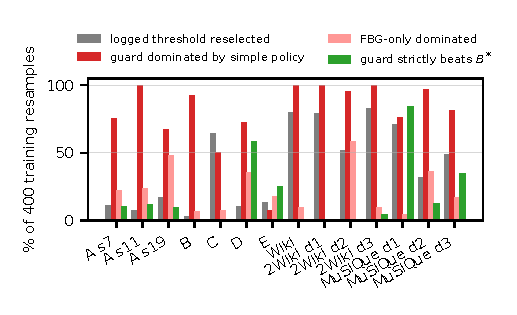
\includegraphics[width=0.6\textwidth]{figures/fig_nested.pdf}
  \caption{Nested refit/reselection over 400 training-episode resamples per
  fully instrumented run. Bars report threshold reselection, simple-policy domination, and
  guarded-policy wins over reselected $B^\star$.}
  \label{fig:supp-nested}
  \Description{Grouped bars for each fully instrumented run showing the share of bootstrap
  replicates that recover the logged threshold, are dominated by a simple policy, or
  beat the reselected fixed-budget comparator.}
\end{figure}

For Table~\ref{tab:supp-nested}, ``dom.'' is the dominated share and
F2/F3/Rep identify the dominating comparator.

\begin{table}[htbp]
\caption{Nested refit/reselection results for the guarded and FBG-only rules.}
\label{tab:supp-nested}
\small
\setlength{\tabcolsep}{3pt}
\begin{tabular}{lrrrrrrrrr}
\toprule
Run & $\theta$ recovered & $\Delta$EM [CI] & C & dom.\,G & dom.\,V & G$\succ B^\star$ & F2 & F3 & Rep \\
\midrule
Corpus s7, A & 11\% & -0.07\,[-0.50,0.50] & 6.24 & 75\% & 22\% & 10\% & 71\% & 6\% & 51\% \\
Corpus s11, A & 8\% & -0.11\,[-0.50,0.25] & 6.07 & 100\% & 24\% & 12\% & 100\% & 4\% & 87\% \\
Corpus s19, A & 17\% & -0.41\,[-1.00,0.25] & 6.52 & 67\% & 48\% & 10\% & 0\% & 18\% & 55\% \\
Corpus s7, B & 3\% & -2.98\,[-3.75,-1.75] & 6.06 & 92\% & 7\% & 0\% & 90\% & 2\% & 24\% \\
Corpus s7, C & 64\% & -3.10\,[-3.50,-1.99] & 6.03 & 50\% & 7\% & 0\% & 0\% & 1\% & 49\% \\
Corpus s7, D & 11\% & +1.01\,[0.25,1.50] & 6.40 & 72\% & 36\% & 58\% & 2\% & 15\% & 72\% \\
Corpus s7, E & 14\% & -0.83\,[-2.25,0.25] & 6.84 & 8\% & 18\% & 25\% & 0\% & 0\% & 7\% \\
2Wiki d1 & 79\% & +0.26\,[0.25,0.26] & 5.56 & 100\% & 1\% & 0\% & 100\% & 0\% & 90\% \\
2Wiki d2 & 52\% & -1.68\,[-2.25,-0.50] & 6.08 & 95\% & 58\% & 0\% & 91\% & 12\% & 32\% \\
2Wiki d3 & 83\% & +0.07\,[-0.25,0.50] & 5.69 & 100\% & 10\% & 4\% & 100\% & 0\% & 29\% \\
MuSiQue d1 & 71\% & -1.83\,[-2.00,-1.75] & 6.57 & 76\% & 5\% & 84\% & 32\% & 0\% & 76\% \\
MuSiQue d2 & 32\% & -0.73\,[-1.00,0.00] & 6.78 & 97\% & 36\% & 13\% & 97\% & 0\% & 28\% \\
MuSiQue d3 & 49\% & -1.17\,[-1.25,-0.75] & 6.55 & 81\% & 17\% & 34\% & 81\% & 0\% & 35\% \\
Wikipedia 25M & 80\% & -0.24\,[-0.25,0.00] & 5.96 & 100\% & 10\% & 0\% & 100\% & 0\% & 92\% \\

\bottomrule
\end{tabular}
\end{table}

Here, $\theta$ recovered is the share reselecting the logged threshold.
$\Delta$EM is guarded minus full-budget EM with a 95\% training-only interval,
and C is guarded calls. Across fully instrumented runs, $B^\star$ ranges from 1 to 4 and the
interval widths are 0.75 to 2.5~EM. FBG-only is dominated less often (7 to 48\%)
because it is frequently cheapest while losing 1.8 to 11.2~EM.
Every resample keeps the questions, logged queries, retrieved evidence,
corpus, preprocessing, and decoder realization fixed. It resamples complete
training chains, then repeats predictor fitting, threshold selection, and
simple-policy selection. The resulting frequencies isolate training and
selection instability rather than full pipeline uncertainty.

\FloatBarrier
\section{Hierarchical view of the corpus-index runs (RQ2)}

\begin{figure}[htbp]
  \centering
  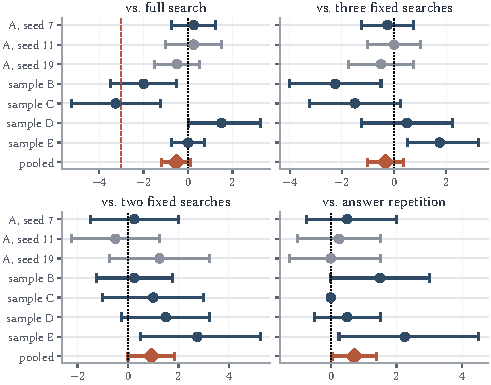
\includegraphics[width=0.62\textwidth]{figures/fig_samples.pdf}
  \caption{Guarded-FBG contrasts across fixed-question reruns (A) and
  independent draws (B to E). Bars are 95\% CIs, diamonds are pooled estimates,
  and the dashed line marks the $-3$~EM margin.}
  \label{fig:samples}
  \Description{Forest plots of guarded-FBG exact-match differences from the
  full budget, fixed-3, fixed-2, and answer repetition across seven runs.}
\end{figure}


\label{supp:hier}

Averaged over the three stochastic runs on question sample A the guarded rule
reaches an equal-weight 25.17~EM at 6.64 versus 9.00 calls. Over all seven
corpus-index runs the equal-weight means are 27.04~EM at 6.67 calls for
guarded FBG, 27.57 at 9.00 for the full budget, 27.36 at 7.00 for fixed-3,
26.32 at 5.77 for repetition, and 25.43 at 5.81 for FBG-only. The
guarded rule is $-0.54$~EM against the full budget at 6.67 versus 9.00 calls,
$-0.32$ against fixed-3 at 0.34 fewer calls, and $-2.14$ for FBG-only
against the full budget.

\begin{table}[htbp]
\caption{Paired EM contrasts across fixed-question reruns, independent
question draws, and the question-clustered pooled analysis.}
\label{tab:supp-hier}
\footnotesize
\setlength{\tabcolsep}{2.4pt}
\begin{tabular}{lrrrrrrr}
\toprule
Contrast & A & B & C & D & E & SD obs/exp & Pooled [CI] \\
\midrule
G $-$ full & -0.00 & -2.00 & -3.25 & +1.50 & +0.00 & 1.87/0.73 & -0.54\,[-1.18,0.11] \\
G $-$ fixed-3 & -0.25 & -2.25 & -1.50 & +0.50 & +1.75 & 1.59/0.80 & -0.32\,[-1.03,0.37] \\
G $-$ fixed-2 & +0.33 & +0.25 & +1.00 & +1.50 & +2.75 & 1.02/0.95 & +0.93\,[0.00,1.86] \\
G $-$ repetition & +0.25 & +1.50 & +0.00 & +0.50 & +2.25 & 0.94/0.69 & +0.71\,[0.04,1.40] \\
V $-$ full & -0.00 & -1.75 & -13.00 & +0.75 & -1.00 & 5.67/1.15 & -2.14\,[-3.06,-1.24] \\
V $-$ fixed-3 & -0.25 & -2.00 & -11.25 & -0.25 & +0.75 & 4.94/1.16 & -1.93\,[-2.87,-1.00] \\
V $-$ fixed-2 & +0.33 & +0.50 & -8.75 & +0.75 & +1.75 & 4.32/1.05 & -0.68\,[-1.57,0.21] \\
\bottomrule
\end{tabular}

\end{table}

\FloatBarrier
\section{Accuracy to cost frontiers for every fully instrumented run}
\label{supp:frontier}

We plot every fully instrumented core cell to show whether the headline
frontier verdict is localized to one dataset or model. The panels cover five
HotpotQA samples, the Wikipedia boundary, and the 2WikiMultihopQA and MuSiQue
draws.

\begin{figure}[htbp]
\centering
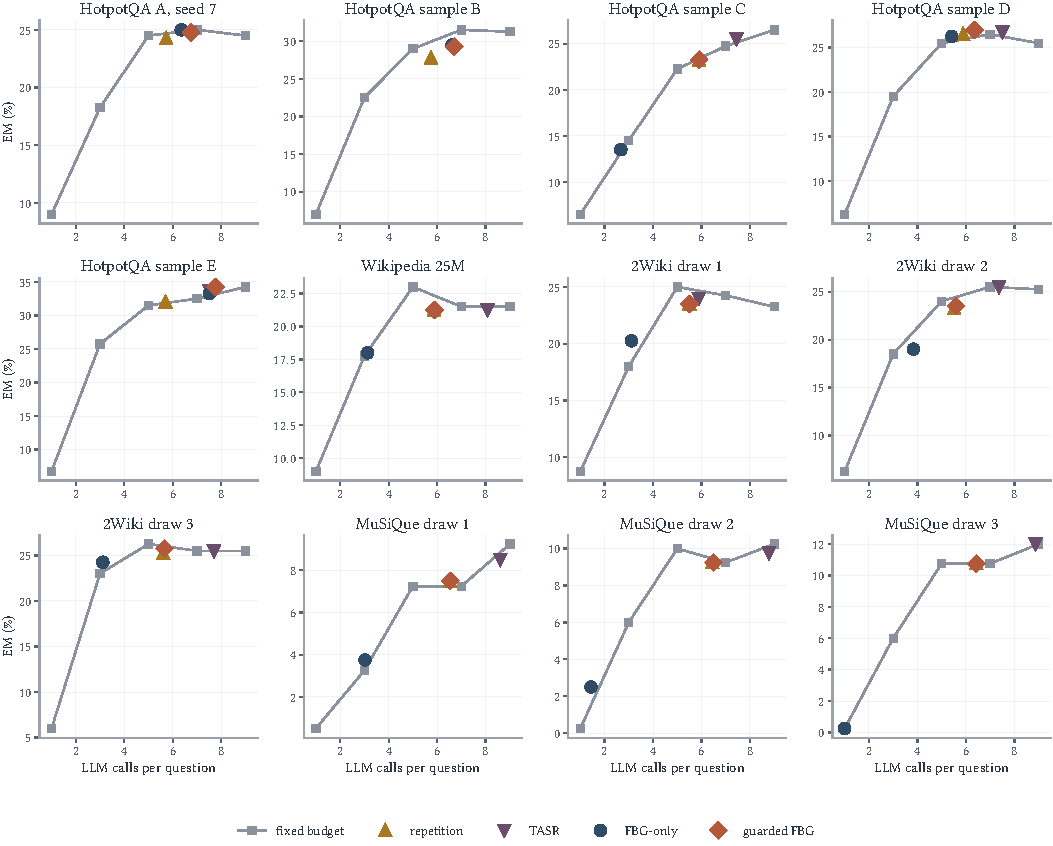
\includegraphics[width=\textwidth]{figures/fig_frontier_all}
\caption{Accuracy-to-call frontiers for fixed budgets, answer repetition,
full TASR, and learned policies in fourteen fully instrumented cells.}
\label{fig:supp-frontier}
\Description{Small-multiple scatter plots of exact-match accuracy versus LLM
calls for simple and learned policies in every fully instrumented retrieval run.}
\end{figure}

\FloatBarrier
\section{Full corpus-confirmation Pareto tables}
\label{supp:corpus}

Here S and C denote searches and exact LLM calls. In is input tokens per
question. Wall is LLM-plus-retrieval seconds per question. Pareto membership
uses EM and calls.

\begin{table}[htbp]
\caption{Primary corpus-wide confirmation ($n{=}400$, question sample A,
seed 7).}
\label{tab:supp-corpus}
\small
\setlength{\tabcolsep}{3pt}
\begin{tabular}{lrrrrrc}
\toprule
Method & EM & S & C & In & Wall & Pareto \\
\midrule
Full budget & 24.5 & 4.00 & 9.00 & 1821 & 5.5 & no \\
Fixed-2 & 24.5 & 2.00 & 5.00 & 775 & 3.1 & yes \\
$B^*{=}3$ & 25.0 & 3.00 & 7.00 & 1282 & 4.3 & no \\
Answer repetition & 24.2 & 2.36 & 5.72 & 1011 & 3.6 & no \\
TASR (full logit rule) & 24.8 & 2.84 & 6.68 & 1233 & 4.0 & no \\
FBG + NLI + repeat guard & 24.0 & 2.52 & 6.03 & 1082 & 3.8 & no \\
Repeat-conditioned gain & 24.5 & 2.89 & 6.78 & 1288 & 4.2 & no \\
FBG value only & 25.0 & 2.67 & 6.35 & 1143 & 3.9 & yes \\
FBG + repeat guard & 24.8 & 2.88 & 6.75 & 1261 & 4.2 & no \\

\bottomrule
\end{tabular}
\end{table}

\FloatBarrier
\section{Call-only full-budget panel}
\label{supp:call-only}

In this call-only panel, CB is closed-book EM. $\Delta$EM is the paired
VoI-minus-ReAct difference with a bootstrap 95\% CI. S is searches per
question, and $\Delta$S is the saving from ReAct's four searches.

\begin{table}[H]
\caption{Frozen-protocol HotpotQA results across nine backbones versus the
full budget in per-question-context cells.}
\label{tab:supp-backbones}
\small
\setlength{\tabcolsep}{4pt}
\begin{tabular}{l r r l l l r r}
\toprule
Backbone & $n$ & CB & ReAct EM\,[CI] & \system\ EM\,[CI] & $\Delta$EM\,[CI] & S & $\Delta$S \\
\midrule
Claude Haiku 4.5 & 140 & 19 & 52.1\,[43.6,60.7] & 50.7\,[42.8,59.3] & -1.4\,[-5.0,2.1] & 1.88 & 53\% \\
Claude Sonnet 4.5 & 140 & 8 & 52.1\,[43.6,60.7] & 53.6\,[45.0,62.1] & +1.4\,[0.0,3.6] & 2.85 & 29\% \\
GPT-oss-120B & 140 & 28 & 57.1\,[48.6,65.7] & 55.7\,[47.1,64.3] & -1.4\,[-4.3,1.4] & 2.49 & 38\% \\
Amazon Nova Lite & 140 & 16 & 54.3\,[45.7,62.9] & 52.9\,[45.0,61.4] & -1.4\,[-3.6,0.0] & 2.94 & 27\% \\
Qwen2.5-3B & 140 & 10 & 38.6\,[30.7,46.4] & 39.3\,[31.4,47.9] & +0.7\,[-3.6,5.0] & 2.56 & 36\% \\
Llama-3.2-3B & 140 & 16 & 39.3\,[31.4,47.9] & 37.9\,[30.0,45.7] & -1.4\,[-6.4,3.6] & 2.21 & 45\% \\
Command-R-35B & 100 & 25 & 51.0\,[41.0,61.0] & 53.0\,[43.0,63.0] & +2.0\,[0.0,5.0] & 2.88 & 28\% \\
Kimi K2.5 & 140 & 28 & 59.3\,[51.4,67.1] & 57.9\,[49.3,66.4] & -1.4\,[-5.0,2.1] & 1.97 & 51\% \\
MiniMax M2.5 & 140 & 21 & 55.7\,[47.9,64.3] & 53.6\,[45.7,62.1] & -2.1\,[-7.1,2.9] & 1.71 & 57\% \\
\bottomrule
\end{tabular}
\end{table}

\begin{table}[H]
\caption{Frozen-protocol replication across datasets in
per-question-context cells. Ref = full-budget ReAct.}
\label{tab:supp-datasets}
\small
\begin{tabular}{l l r cc cc c}
\toprule
& & & \multicolumn{2}{c}{ReAct} & \multicolumn{2}{c}{\system} & \\
\cmidrule(lr){4-5}\cmidrule(lr){6-7}
Dataset & Backbone & $n$ & EM & S & EM & S & $\Delta$S \\
\midrule
2Wiki & Qwen2.5-3B & 140 & 28.6 & 4.0 & 28.6 & 2.60 & 35\% \\
MuSiQue & Qwen2.5-3B & 140 & 13.6 & 4.0 & 12.1 & 2.04 & 49\% \\
MuSiQue & Llama-3.2-3B & 100 & 18.0 & 4.0 & 16.0 & 2.43 & 39\% \\
\bottomrule
\end{tabular}
\end{table}

\begin{table}[H]
\caption{Adaptive-retrieval baselines versus frozen \system\ on the HotpotQA
Qwen2.5-3B baseline-implementation cell ($n{=}140$).}
\label{tab:supp-baselines}
\small
\begin{tabular}{l r r r}
\toprule
Method & EM & S & $\Delta$S \\
\midrule
\;Self-RAG (released 7B) & 7.9 & 0.56 & \\
\;FLARE-direct & 34.3 & 1.66 & \\
\;SKR$_{\mathrm{knn}}$ & 27.1 & 1.00 & \\
\;Adaptive-RAG (trained) & 37.9 & 3.81 & \\
\;ReAct (full budget) & 38.6 & 4.00 & \\
\;\textbf{VoI-Search} & \textbf{39.3} & \textbf{2.56} & \textbf{36\%} \\
\addlinespace
\bottomrule
\end{tabular}
\end{table}

\FloatBarrier
\section{Expanded deterministic reference family}
\label{supp:deterministic-controls}
This retrospective check adds evidence-growth saturation to all fixed budgets
and answer repetition in 14 fully instrumented cells. Thresholds in
$\{0,1,2,3\}$ are selected on training chains only, using the same one-EM
admissibility band and lower-call preference as the earlier diagnostic.
The control stops after at least one search when newly retained units do not
exceed the selected threshold. It uses already logged features and makes no
additional LLM calls. Training and test question identifiers are disjoint.

We recompute the observed simple-policy hull for calls, input tokens, and a
wall-time sensitivity coordinate. The latter adds the measured local CPU
cost of applying the control (0.26 to 0.34 microseconds per question, 100
repetitions) to historical model and retrieval timings. These mixed-hardware
numbers are a sensitivity analysis, not a new end-to-end latency benchmark.

Table~\ref{tab:deterministic-controls} reports mean paired EM gaps across
cells. A single 84-contrast family covers 14 cells, two FBG policies, and three
cost coordinates. We use 10,000 Gaussian multiplier draws, sharing each
question's weight across cells and coordinates, and the 95th percentile of
the maximum absolute standardized contrast (3.140). These exploratory bands
condition on fitted policies and observed hull vertices and mixture weights. They do not include training or frontier-reselection uncertainty. All 84
bands include zero, which does not establish equivalence. The original
frozen 26-cell analysis remains unchanged.

\begin{table}[htbp]
\centering\small
\caption{Expanded-reference matched-cost sensitivity.}
\label{tab:deterministic-controls}
\begin{tabular}{llrr}
\toprule
Policy & Cost coordinate & Mean EM gap & Win/unresolved/loss\\
\midrule
Guarded & Calls & $-0.68$ & 0/14/0 \\
Guarded & Input tokens & $-0.72$ & 0/14/0 \\
Guarded & Wall-time proxy & $-0.69$ & 0/14/0 \\
FBG-only & Calls & $-0.07$ & 0/14/0 \\
FBG-only & Input tokens & $-0.09$ & 0/14/0 \\
FBG-only & Wall-time proxy & $-0.05$ & 0/14/0 \\

\bottomrule
\end{tabular}
\end{table}

\FloatBarrier
\section{Fresh eight-search extension}
\label{supp:long-horizon}
We prospectively froze a bounded extension on November 18, 2026 before
collecting model outputs. From HotpotQA distractor validation, we exclude
all question identifiers recoverable from the archived training and test
records, then shuffle with seed 212613 and select 120 training and 200 test
questions. The two sets are disjoint. The artifact records their identifiers,
the dataset checksum, and the frozen protocol. Policy fitting and five-fold
chain cross-fitting use 90 training chains, with 30 reserved and unused for
this stopping analysis, preserving the original calibration split.

Claude Haiku 4.5 (\texttt{claude-haiku-4-5-20251001}, temperature zero)
produces an initial answer and eight search-query/answer pairs per question.
Queries adapt to accumulated evidence using the submitted prompts. Retrieval
uses SQLite FTS5/BM25 over 269,558 deduplicated sentence units from the public
validation contexts, with no gold-support filtering. We replay stopping at
horizons four and eight on these same fresh trajectories. This is new
longer-horizon evidence, not a jointly learned query-and-stop policy or a
replication on the original nine backbones.

At each horizon, we refit the original clipped-FBG and current-error heads,
select the guarded threshold by training-chain cross-fitting, and use that
threshold for both guarded and FBG-only stopping as in the original protocol.
The reference family includes every fixed budget, answer repetition, and
training-selected evidence growth. Both training-selected fixed budgets use
the full horizon. Table~\ref{tab:long-horizon} reports every horizon/policy
combination. D and I are descriptive categories, not inferential conclusions.

\begin{table}[htbp]
\centering\small
\caption{Fresh-question longer-horizon check ($n=200$).}
\label{tab:long-horizon}
\begin{tabular}{rlrrrrrr}
\toprule
Horizon & Policy & $B^\star$ & EM & Calls & Class & Gap & Simultaneous CI\\
\midrule
4 & Guarded & 4 & 53.50 & 5.71 & D & $-0.85$ & $[-4.24,+2.53]$ \\
4 & FBG-only & 4 & 55.00 & 4.91 & I & $+1.69$ & $[-2.10,+5.47]$ \\
8 & Guarded & 8 & 55.00 & 8.24 & D & $+0.00$ & $[-2.43,+2.43]$ \\
8 & FBG-only & 8 & 55.50 & 8.19 & I & $+0.50$ & $[-2.22,+3.22]$ \\

\bottomrule
\end{tabular}
\end{table}

At horizon eight, guarded FBG reaches 55.0 EM at 8.24 calls and FBG-only
reaches 55.5 EM at 8.19 calls. Full-budget EM is 53.5 at horizon four and
55.0 at horizon eight. Their paired difference is 1.5 EM points, with an
unadjusted percentile-bootstrap 95\% interval $[0.0,3.5]$. The prefix oracle
is 61.5 EM at both horizons. The extra searches thus improve the final
answer on average in this sample without raising the observed oracle ceiling.

The 12-contrast exploratory family covers two horizons, two policies, and
calls, provider-reported input tokens, and measured request-plus-retrieval
latency. We use 10,000 shared-question Gaussian multiplier draws and a
maximum absolute standardized-contrast critical value of 2.428. The bands
condition on fitted policies and observed hull vertices and mixture weights,
without frontier reselection or training uncertainty. All 12 contain zero.
In particular, the eight-search equal-call FBG-only gap is 0.50 EM points
with a conditional simultaneous interval $[-2.22,3.22]$. This limited check
does not establish equivalence or rule out longer-horizon gains.

Collection completed all 320 trajectories and 5,440 model requests with
zero recorded failures. A separate connectivity probe adds one request.
Provider usage totals 1,601,333 input and 86,545 output tokens including the
probe, giving an estimated list-price cost of \$2.034058 at \$1 and \$5 per
million tokens, respectively. This is below the authorized \$25 cap and is
not an invoice. Eight concurrent workers affect latency, so these timings
are specific to this collection. The record includes prefix costs, queries,
answers, retained evidence, features, selected thresholds, and all outcomes.

\bibliographystyle{ACM-Reference-Format}
\bibliography{references}
\end{document}
